
\chapter{Method 1: Direct intersection}
\label{ch:direct_intersection}

The first presented method to extract a triangulated surface from the VML's data model is by directly processing the stored triangles inside the VML's regular grid.
This approach is the most naive, computationally intensive, but, in theory, most accurate.
It is conceptually equivalent to directly intersecting the mesh of the stock with each swept volume mesh.
Boolean operations on triangle meshes are already available in most CAD kernels.
However, these kernels usually require the meshes to be closed.
Due to the triangle elimination strategy using cell classification, \cf section \ref{sec:classification}, the meshes stored in the regular grid are no longer closed.
Thus, regular CAD kernels cannot be used to intersect the meshes maintained by the VML and a custom mesh intersection algorithm has been developed.
The idea of this approach is based on a paper about finding and deforming the intersection between two meshes as well as applying textures to those regions to increase the realism in computer graphics, \ie computer games \cite{mesh_intersection}.

\section{Concept}
\label{sec:direct_intersection_concept}

Every time a swept volume is added to the VML, a unique id is generated and assigned to each of the swept volume's triangles before they are mapped to the cells of the regular grid.
As the stock is internally treated as a swept volume, by inverting the surface normals, all stock triangles are also assigned a unique id.
These ids allow to separate the triangles contained in the regular grid into the previous swept volumes, referred to as structures.
The separated structures are processed in pairs.
Each pair is united into a new structure.
The union of the two structure meshes is calculated by intersecting each triangle of one mesh with each triangle of the other mesh.
If two triangles intersect, the intersection line is recorded for both triangles.
After intersection, each triangle with intersection lines is split along these lines, retriangulated and replaced by the triangles resulting from the retriangulation.
All previous intersection lines are now edges of new triangles.
Each triangle of one structure is then tested against the other structure, whether the triangle is inside or outside the other structure, \eg by casting a ray from the triangle to the other structure.
As all triangles intersecting the opposite structure have been split, this property should be unambiguously determinable for each triangle.
By removing all triangles inside the opposite structure, the remaining triangles form a new surface which corresponds to the union of both structures.
This new structure is then again pairwise united with other structures until only one structure is left, \ie all structures are reduced to one.
This final structure is the reconstructed surface of the VML's data model.
Figure \ref{fig:cube2} demonstrates this workflow by the example of intersecting a cube with a cuboid.

\begin{figure}
	\centering
	\begin{subfigure}[t]{0.3\textwidth}
		\centering
		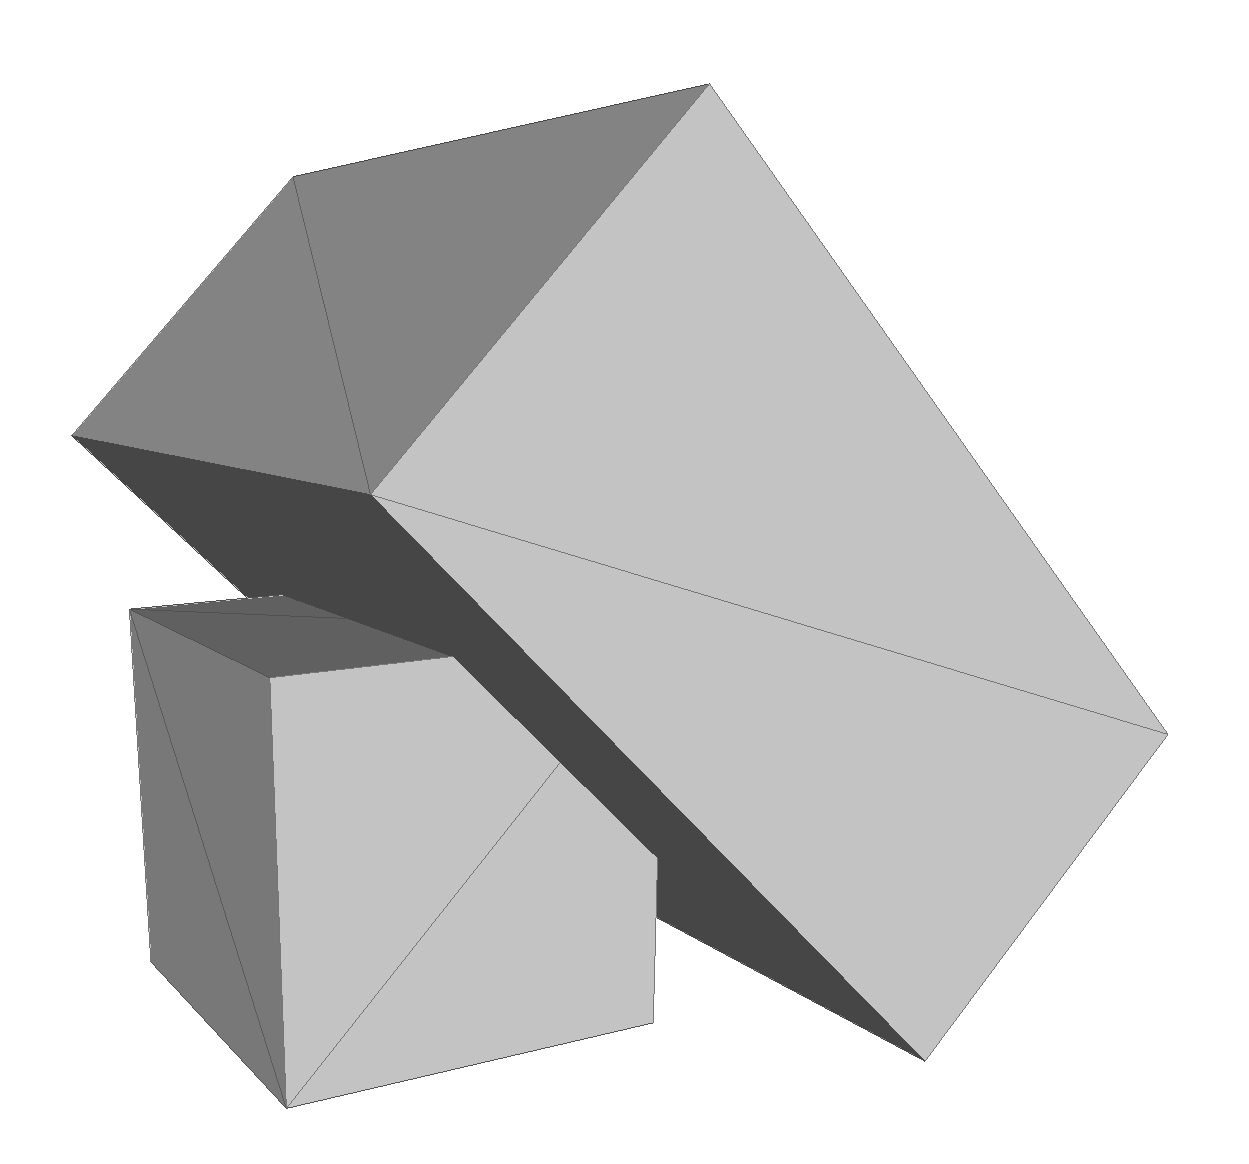
\includegraphics[width=\textwidth]{images/cube2_stock_sv}
		\caption{Stock and SV}
		\label{fig:cube2_stock_sv}
	\end{subfigure}
	\begin{subfigure}[t]{0.3\textwidth}
		\centering
		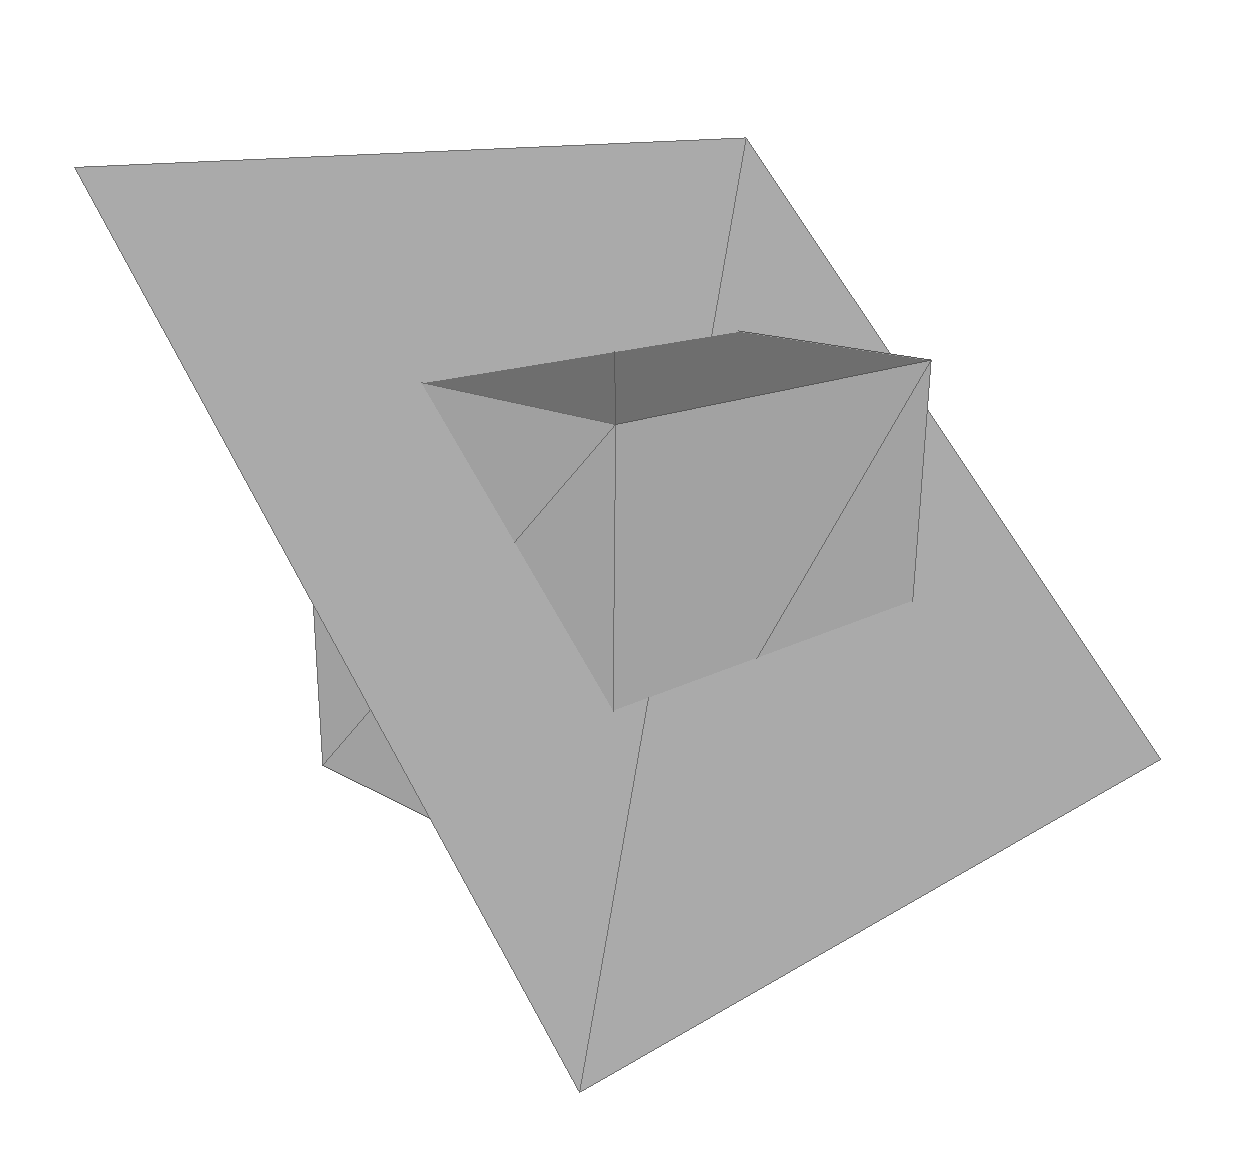
\includegraphics[width=\textwidth]{images/cube2_classified}
		\caption{VML}
		\label{fig:cube2_classified}
	\end{subfigure}
	\begin{subfigure}[t]{0.3\textwidth}
		\centering
		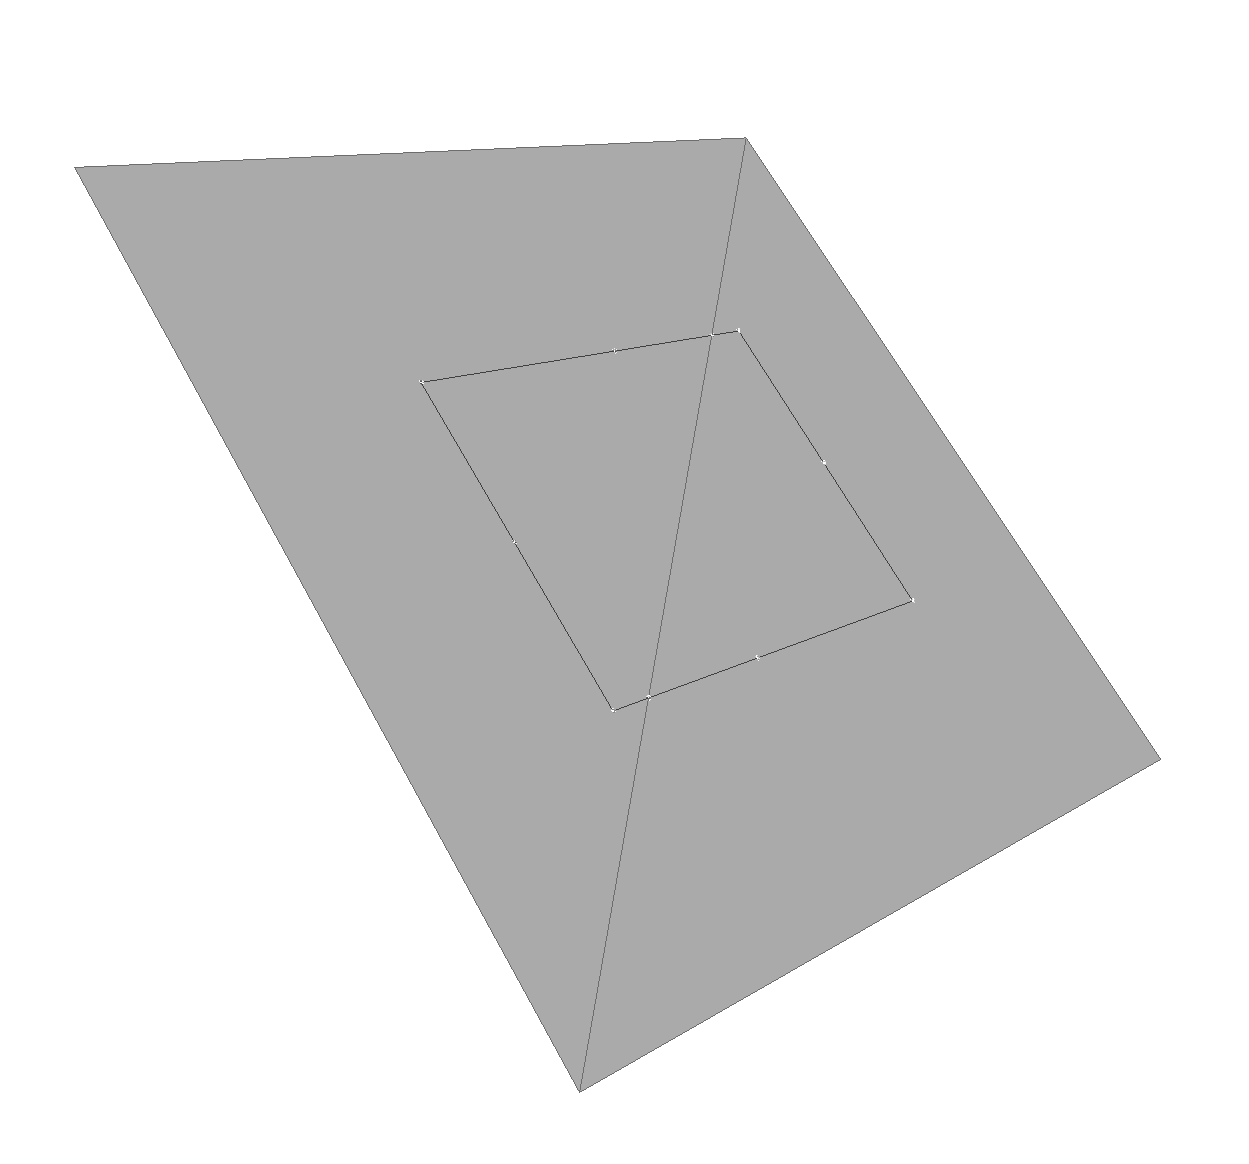
\includegraphics[width=\textwidth]{images/cube2_constraints}
		\caption{Intersections}
		\label{fig:cube2_constraints}
	\end{subfigure}
	\begin{subfigure}[t]{0.3\textwidth}
		\centering
		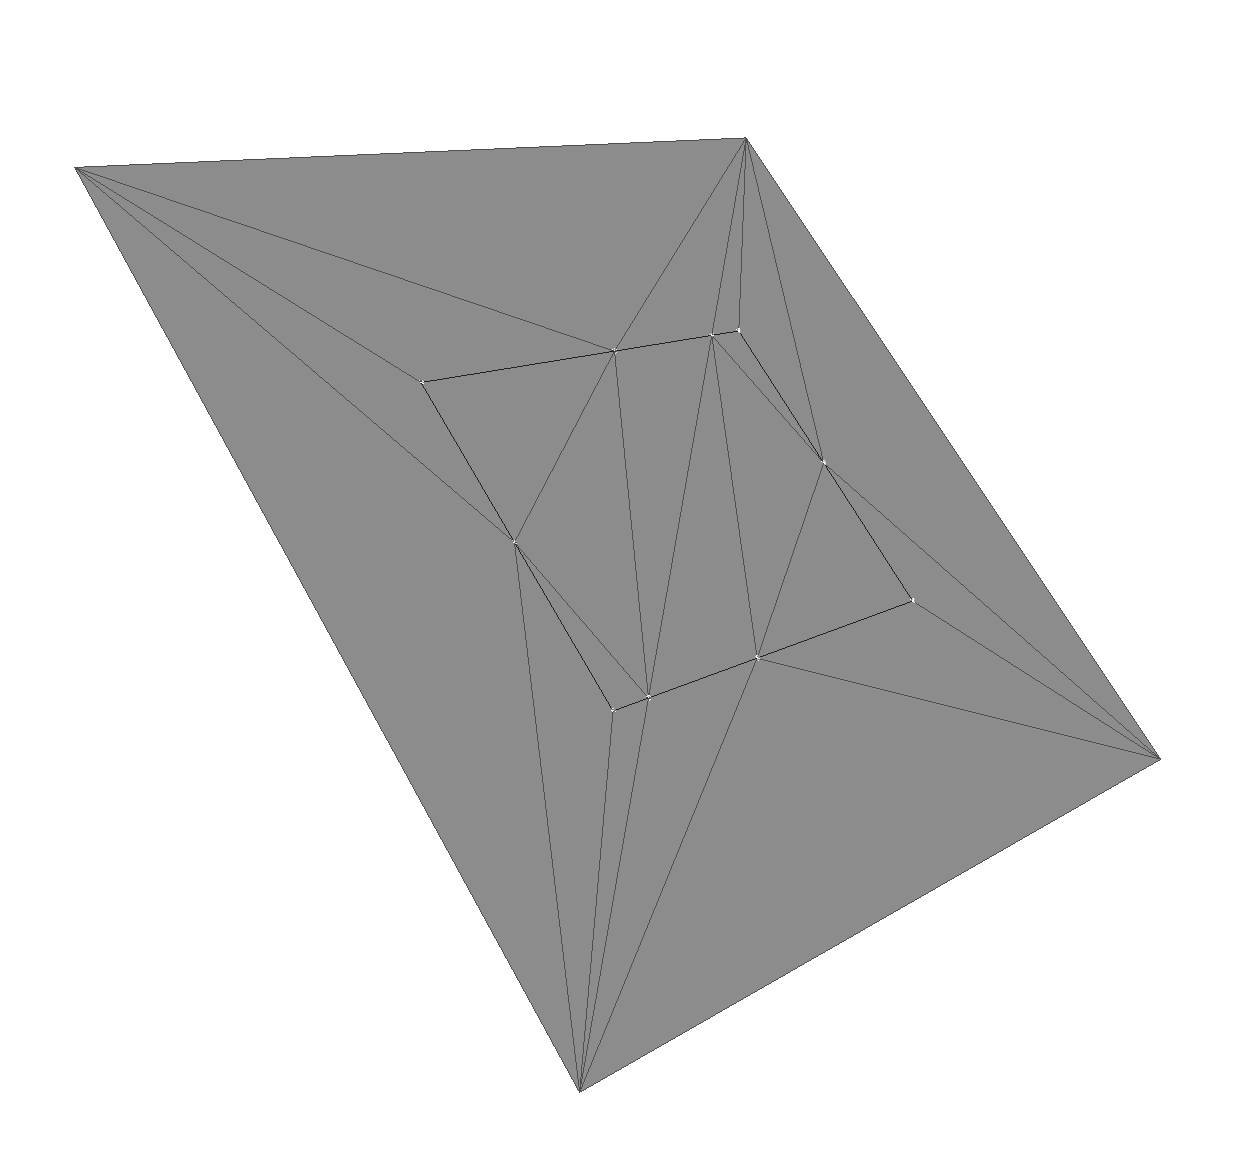
\includegraphics[width=\textwidth]{images/cube2_retriangulated}
		\caption{Retriangulation}
		\label{fig:cube2_retriangulated}
	\end{subfigure}
	\begin{subfigure}[t]{0.3\textwidth}
		\centering
		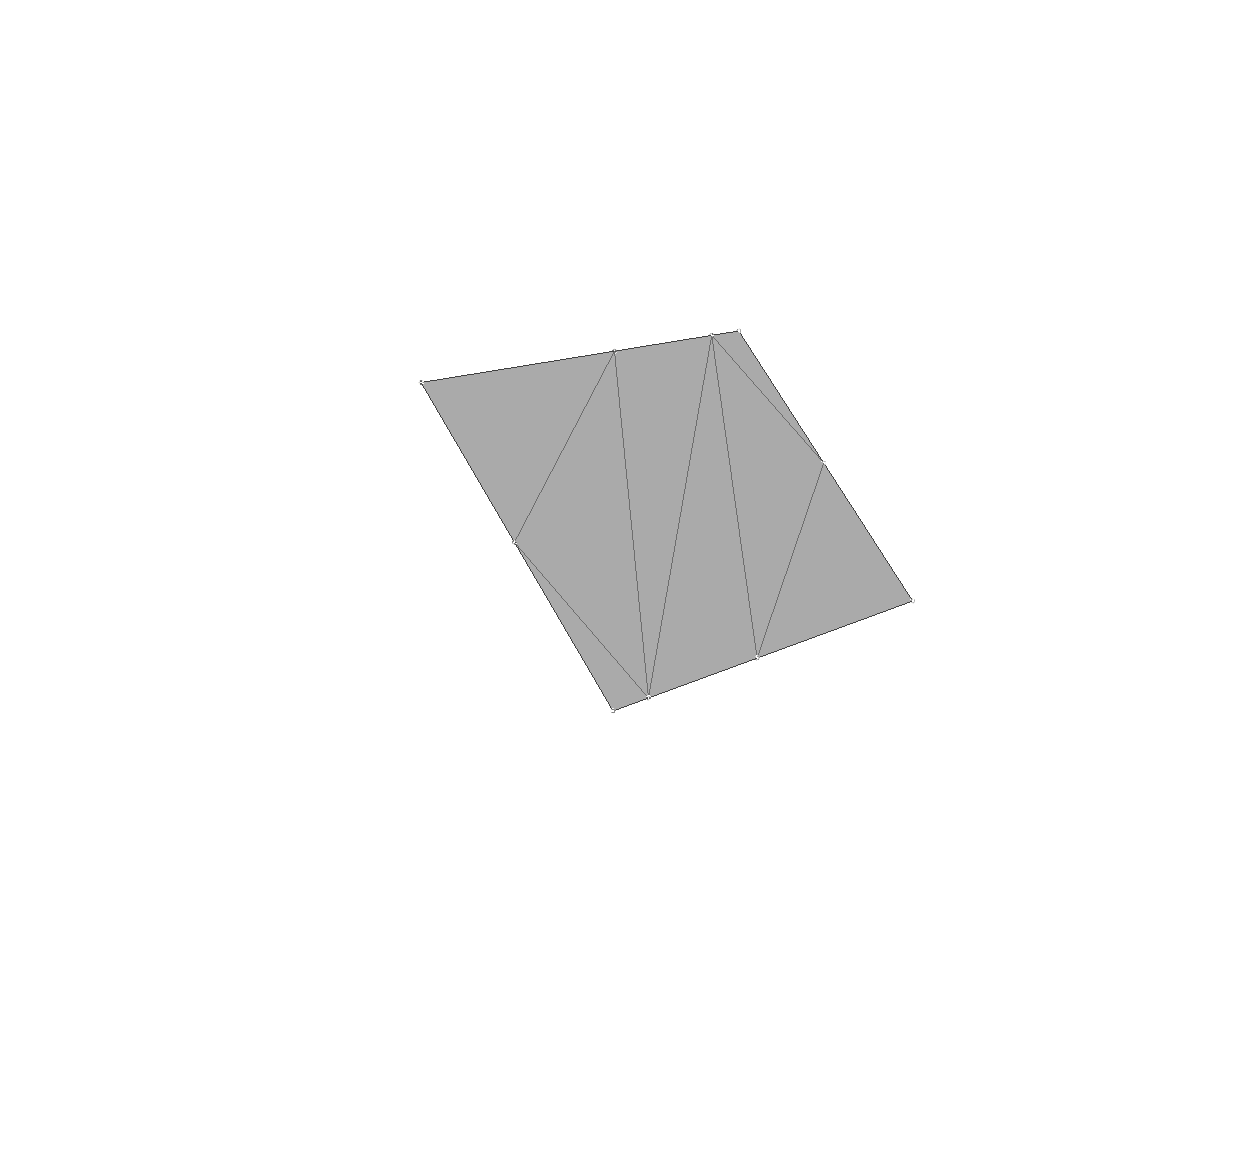
\includegraphics[width=\textwidth]{images/cube2_eliminated}
		\caption{Inside test}
		\label{fig:cube2_eliminated}
	\end{subfigure}
	\begin{subfigure}[t]{0.3\textwidth}
		\centering
		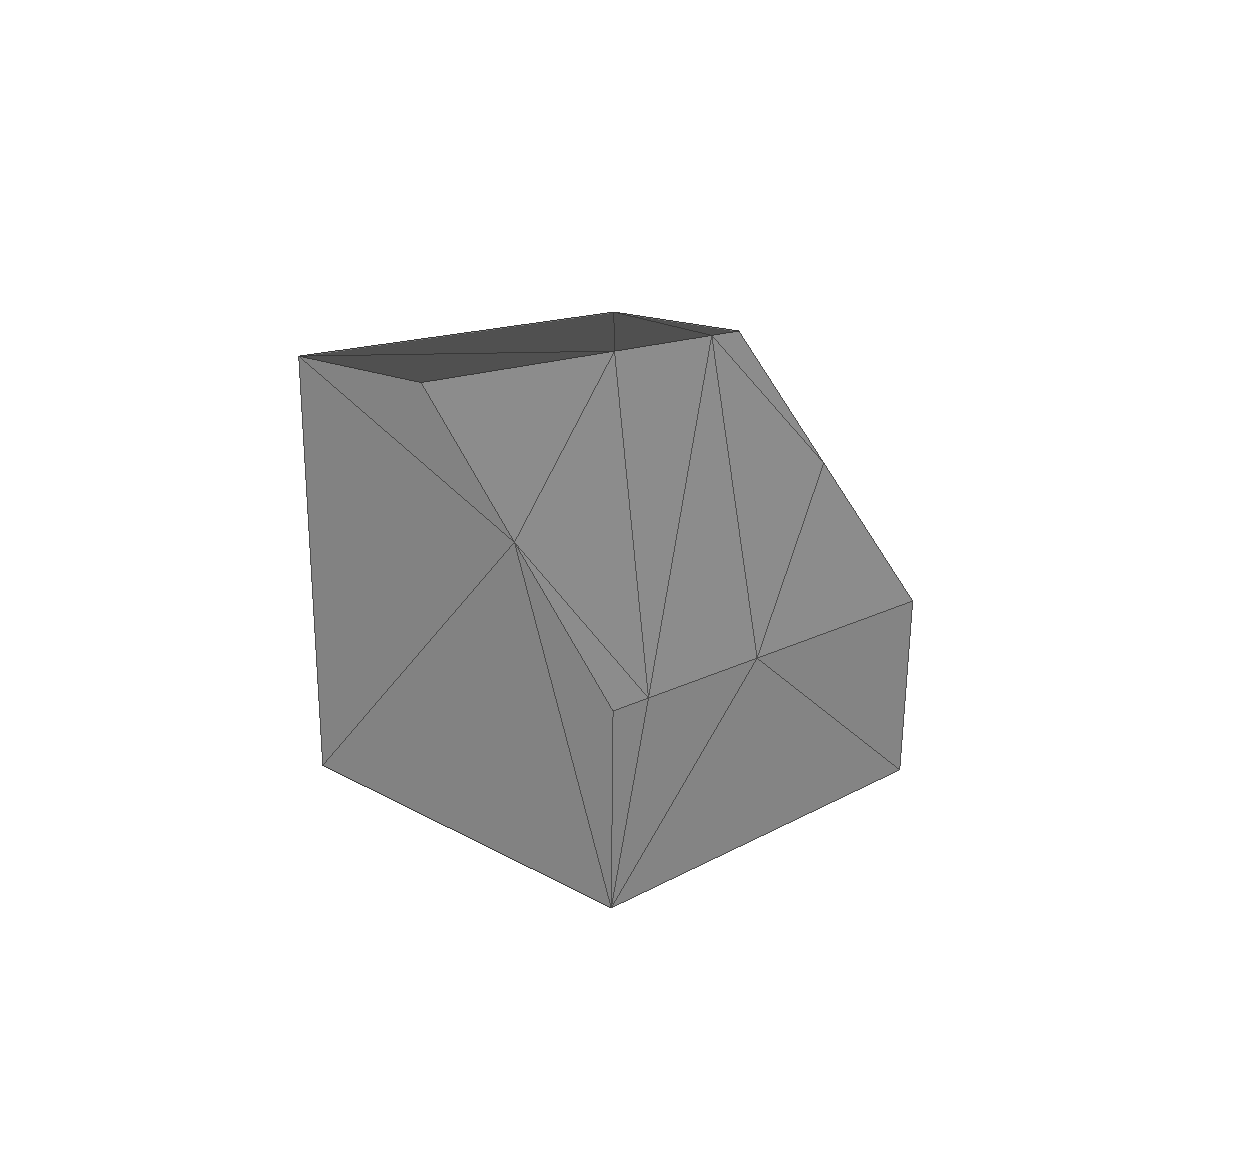
\includegraphics[width=\textwidth]{images/cube2_result}
		\caption{Result}
		\label{fig:cube2_result}
	\end{subfigure}
	\caption{
		Surface reconstruction from the VML's data model by the example of intersecting a cube and a cuboid.
		Figure \ref{fig:cube2_stock_sv} shows the cubic stock, in the lower left, and a tilted cuboid as swept volume, in the upper right.
		Figure \ref{fig:cube2_classified} shows the classification result when these two solids are mapped into the VML's regular grid.
		Most of the swept volume's triangles have been removed.
		When intersecting both structures, \ie swept volume and stock triangles, all intersection lines per triangle are recorded.
		Regarding the swept volume's triangles, these are shown in figure \ref{fig:cube2_constraints}.
		The triangles are then retriangulated with respect to those intersections as shown in figure \ref{fig:cube2_retriangulated}.
		Afterwards, each triangle is tested against the other structure, whether they are inside and can be removed.
		The result of testing the retriangulated swept volume's triangles against the stock is shown in figure \ref{fig:cube2_eliminated}.
		The retriangulation and inside test is analogously done for the stock structure.
		Finally, the reconstructed surface is the union of the remaining triangles, figure \ref{fig:cube2_result}.
	}
	\label{fig:cube2}
\end{figure}


\section{Implementation}
\label{sec:direct_intersection_implementation}

Due to the regular grid's classification, \cf section \ref{sec:classification}, triangles might have been removed and, consequently, the structures put together from the regular grid's cells may no longer be closed meshes.
As it turns out, the test whether a triangle is inside another structure may fail if the tested structure is not a closed mesh, a common case.
An example of such an issue is shown in figure \ref{fig:inside_test_error}.
%
\begin{figure}
	\centering
	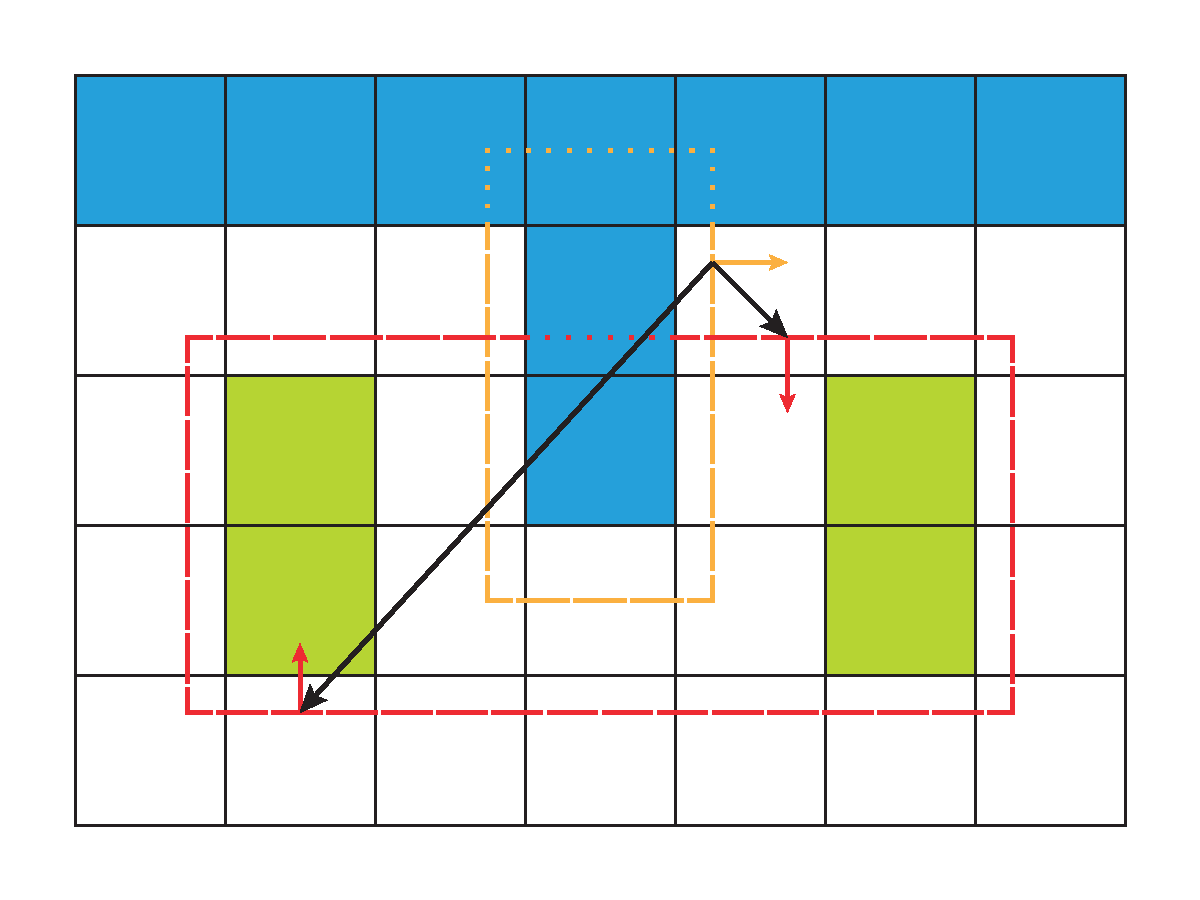
\includegraphics[width=0.8\textwidth]{inside_test_error}
	\caption{
		Testing if a triangle of one structure is inside another structure using a ray.
		Due to triangle elimination, the ray can miss removed structures, \eg when traversing outside cells, causing the inside test to fail, \cf left ray.
		As structures are guaranteed to be closed within a cell, this test is only valid within a cell, \cf right ray.
	}
	\label{fig:inside_test_error}
\end{figure}
%
A triangle is tested against a structure by using a ray.
This ray is shot from an arbitrary point on the triangle, which does not lie on an edge, \eg the triangle's centroid, to an arbitrary point on a triangle of the other structure.
If the ray does not intersect the other structure on its way, a comparison of the ray's direction with the normal of the targeted triangle determines whether the ray's origin, \ie the centroid of the tested triangle, is inside the other structure or not.
However, as classification might eliminate triangles, the ray could potentially intersect triangles of the structure which have been removed, \cf left ray in figure \ref{fig:inside_test_error}.
The regular grid only guarantees closed meshes within a cell.
To circumvent this issue, the inside test for a triangle must be conducted within a cell.

In general, intersecting each triangle of a structure against each other triangle of another structure is an expensive undertaking.
The cost of this operation is $\mathcal{O}(n^2)$, assuming both structures have $n$ triangles.
Intersecting the structures at the level of each cell greatly reduces the value of $n$.
Unfortunately, many triangles usually span the bounding box of a cell and are duplicated in each encompassed cell.
To avoid duplicates or overlapping triangles when combining results from neighboring cells, all triangles of a cell have to be clipped against the cell's bounding box.
This step can be done before or after intersecting the structures of a cell, but always before starting to eliminate triangles against the opposite structure.

An abstracted algorithm of this reconstruction approach is shown in algorithm \ref{alg:direct_intersection}.
The following sections discuss details of this algorithms and follow the order of subroutines/functions which are not yet defined.
The only exception is the \textproc{SeparateStructures} routine, which only groups the incoming triangles by their structure id.
It returns a list of structures, where each structure is a set of triangles.

\begin{algorithm}
	\centering
	\begin{algorithmic}[1]
		\Function{DirectIntersection}{$\var{grid}$}
			\State $\var{result} \gets \varnothing$
			\ForAll{$\var{c} \in \var{grid.cells}$}
				\If{$\var{c.classification} = \var{surface}$}
					\State $\var{structures} \gets \Call{SeparateStructures}{\var{c.triangles}}$
					\If{$\left\vert{\var{structures}}\right\vert = 1$}
						\State $\var{result} \gets \var{result} \cup \Call{ClipStructure}{\var{structures.pop()}, \var{c.aabb}}$
					\ElsIf{$\left\vert{\var{structures}}\right\vert > 1$}
						\State $\var{acc} \gets \var{structures.pop()}$
						\While{$\left\vert{\var{structures}}\right\vert > 0$}
							\State $\var{s} \gets \var{structures.pop()}$
							\State $\var{acc} \gets \Call{UnionStructure}{\var{acc}, \var{s}, \var{c.aabb}}$
						\EndWhile
						\State $\var{result} \gets \var{result} \cup \var{acc}$
					\EndIf
				\EndIf
			\EndFor
			\State \Return $\var{result}$
		\EndFunction
		\\
		\Function{UnionStructure}{$\var{s_1}, \var{s_2}, \var{cellBox}$}
			\ForAll{$\var{s} \in \{\var{s_1}, \var{s_2\}}$}
				\State $s \gets \Call{ClipStructure}{\var{s}, \var{cellBox}}$
			\EndFor
			\State $\var{lines} \gets \var{map()}$ \Comment{maps each triangle to a set of lines}
			\ForAll{$(\var{t_1}, \var{t_2}) \in \var{s_1} \times \var{s_2}$}
				\State $\var{l} \gets \Call{IntersectTriangles}{\var{t_1}, \var{t_2}}$
				\If{$\var{l}$} \Comment{no intersection line may be found}
					\State $\var{lines}(\var{t_1}) \gets \var{lines}(\var{t_1}) \cup \{\var{l}\}$
					\State $\var{lines}(\var{t_2}) \gets \var{lines}(\var{t_2}) \cup \{\var{l}\}$
				\EndIf
			\EndFor
			\ForAll{$\var{s} \in \{\var{s_1}, \var{s_2}\}$}
				\State $\var{s'} \gets \varnothing$
				\ForAll{$\var{t} \in \var{s}$}
					\State $\var{s'} \gets \var{s'} \cup \Call{SplitTriangle}{\var{t}, \var{lines}(\var{t})}$
				\EndFor
				\State $\var{s} \gets \var{s'}$
			\EndFor
			\State $\var{result} \gets \varnothing$
			\ForAll{$(\var{s}, \var{s'}) \in \{(\var{s_1}, \var{s_2}), (\var{s_2}, \var{s_1})\}$}
				\ForAll{$\var{t} \in \var{s}$}
					\If{$\neg \Call{IsTriangleInsideStructure}{\var{t}, \var{s'}}$}
						\State $\var{result} \gets \var{result} \cup \{\var{t}\}$
					\EndIf
				\EndFor
			\EndFor
			\State \Return $\var{result}$
		\EndFunction
	\end{algorithmic}
	\caption{
		Abstract workflow of the surface extraction using direct intersection of the VML's stored structures.
	}
	\label{alg:direct_intersection}
\end{algorithm}


\subsection{Clipping}
\label{sec:clipping}

Clipping triangles against the bounding box of a cell is necessary to avoid duplicated or invalid surfaces.
In cases where triangles span multiple cells, the VML duplicates each triangle into each cell it encompasses.
During intersection, only a triangle's intersections with structures of the current cell are recorded, although the triangle might be intersected by additional geometry in neighboring cells.
Therefore, after splitting, parts of the triangle which are outside the current cell are never split, might pass the inside test as a whole and remain as additional triangles outside the actual surface or remain colinear with surface triangles from neighboring cells.
To circumvent these issues, all triangles of a cell have to be clipped either before or after intersecting the two structures in \textproc{UnionStructure}.

Algorithms for clipping triangles against a bounding box are found in literature.
A well-known examples is the Sutherland-Hodgeman algorithm for polygon clipping \cite{polygon_clipping}.
Although further algorithms exist, \eg Weiler-Artherton, Vatti or Greiner-Hormann, which are either faster, more robust or have fewer restrictions on their input, the Sutherland-Hodgeman algorithm is characteristically simple.
In particular, it clips any polygon against any convex clip polygon by iteratively clipping it against infinitely extended lines along each edge of the clip polygon.
Despite being initially designed for 2 dimensions, the algorithm easily extends to higher dimensions.

For clipping triangles against the bounding box of a cell, a 3-dimensional version of the Sutherland-Hodgeman algorithm is needed.
Algorithm \ref{alg:clip} shows a pseudocode implementation of the \textproc{ClipStructure} routine which is based on the Sutherland-Hodgeman algorithm to clip all structure triangles against the bounding box of a cell.
%
When clipping a structure against a bounding box, each individual triangle of the structure is clipped separately.
The result of clipping a single triangle may be the same triangle, a set of new triangles or even no triangle at all.
The resulting triangles after clipping, if any, are collected to form the new, clipped structure.

The Sutherland-Hodgeman algorithm clips against a convex polygon, or its equivalent in higher dimensions, \ie a polytope, by iteratively clipping against each side.
In case of a bounding box, the input polygon has to be clipped against each of the six sides of the cell.
These sides are extended and described as planes by specifying a normal vector and the plane's distance to the origin.
The six planes built from a cell's bounding box are given in the \textproc{ClipPolygonAABB} function of algorithm \ref{alg:clip}.
The input polygon itself is represented as an ordered list of vertices, where each pair of adjacent vertices form an edge of the polygon, including the last and the first vertex as a pair.
The order of the vertices remains the sames during the clipping process, but vertices may be removed or additional ones added.
The final vertex list, after clipping against all planes, needs to be triangulated again.
As the clipping volume, \ie the cell's bounding box, is convex, the resulting clipped polygon is also convex.
Therefore, the list of vertices can be simply triangulated into a fan by selecting one vertex and emitting a triangle for every adjacent pair of vertices excluding the selected vertex, where each triangle is built from the pair and the selected vertex.
Note that in some edge cases, duplicate vertices may be generated.
Thus, duplicates should be removed from the result vertex list before passing it to the triangulation subroutine.

The core routine of the clipping procedure is clipping the list of vertices against a single plane.
Initially, an empty list of result vertices is created.
For each of the polygon's vertices, the signed distance to the clipping plane is calculated.
The distance of each vertex is compared with the distance of its preceding vertex.
If the signs of the distances are different, the edge represented by the current vertex and its predecessor intersects the clipping plane.
In this case, the intersection point with the clipping plane is calculated, \cf algorithm \ref{alg:clip} for details, and the point is added to the result list.
If the distance of the current vertex is positive, the vertex itself is inside the clipping volume and is also added to the result list.
After all vertices have been processed, the result list is return, representing the clipped polygon again as an ordered list of its vertices.

\begin{algorithm}
	\centering
	\begin{algorithmic}[1]
		\Function{ClipStructure}{$\var{s}, \var{aabb}$}
			\State $\var{s'} \gets \varnothing$
			\ForAll{$\var{t} \in \var{s}$}
				\State $\var{s'} \gets \var{s'} \cup \Call{ClipPolygonAABB}{\var{t.vertices}, \var{aabb}}$
			\EndFor
			\State \Return $\var{s'}$
		\EndFunction
		\\
		\Function{ClipPolygonAABB}{$\var{vertices}, \var{aabb}$}
			\State $\var{vertices} \gets \Call{ClipPolygonPlane}{\var{vertices}, \var{Vertex}( 1, 0, 0), \var{aabb.lower.x}}$
			\State $\var{vertices} \gets \Call{ClipPolygonPlane}{\var{vertices}, \var{Vertex}(-1, 0, 0), \var{aabb.upper.x}}$
			\State $\var{vertices} \gets \Call{ClipPolygonPlane}{\var{vertices}, \var{Vertex}( 0, 1, 0), \var{aabb.lower.y}}$
			\State $\var{vertices} \gets \Call{ClipPolygonPlane}{\var{vertices}, \var{Vertex}( 0,-1, 0), \var{aabb.upper.y}}$
			\State $\var{vertices} \gets \Call{ClipPolygonPlane}{\var{vertices}, \var{Vertex}( 0, 0, 1), \var{aabb.lower.z}}$
			\State $\var{vertices} \gets \Call{ClipPolygonPlane}{\var{vertices}, \var{Vertex}( 0, 0,-1), \var{aabb.upper.z}}$
			
			\State \Return $\Call{Trianglulate}{\Call{Unique}{\var{vertices}}}$
		\EndFunction
		\\
		\Function{ClipPolygonPlane}{$\var{vertices}, \var{n}, \var{d}$}
			\State $\var{result} \gets \var{array}()$
			\State $\var{prev} \gets |\var{vertices}| - 1$
			\State $\var{prevDist} \gets \var{vertices_{prev}} * \var{n} - \var{d};$
			\For{$\var{i} \gets 0, \dots, |\var{vertices}| - 1$}
				\State $\var{dist} \gets \var{vertices_i} * \var{n} - \var{d}$;
				\If{$(\var{dist} < 0 \wedge \var{prevDist} \geq 0) \vee (\var{dist} \geq 0 \wedge \var{prevDist} < 0)$}
					\State $\var{edge} \gets (\var{vertices_i} - \var{vertices_{prev}})$
					\State $\var{edge} \gets \var{edge} * \frac{\var{dist}}{\var{n} * \var{edge}}$
					\State $\var{v} \gets \var{vertices_i} - \var{edge}$
					\State $\var{result.add}(\var{v})$
				\EndIf
				\If{$\var{dist} \geq 0$}
					\State $\var{result.add}(\var{vertices_i});$
				\EndIf
				\State $\var{prev} \gets i$;
				\State $\var{prevDist} \gets \var{dist}$;
			\EndFor
			\State \Return $\var{result}$
		\EndFunction
		\\
		\Function{Triangulate}{$\var{vertices}$}
			\State $\var{result} \gets \varnothing$
			\If{$|vertices| \geq 3$}
				\State $\var{c} \gets \var{loop_0}$
				\For{$\var{i} \gets 2, \dots, |\var{vertices}| - 1$}
					\State $\var{result} \gets \var{result} \cup \{\var{Triangle}(\var{c}, \var{vertices_{i - 1}}, \var{vertices_i})\}$
				\EndFor
			\EndIf
			\State \Return $\var{result}$
		\EndFunction
	\end{algorithmic}
	\caption{
		A Sutherland-Hodgeman algorithm variant for clipping polygons against a bounding box in 3 dimensions.
	}
	\label{alg:clip}
\end{algorithm}



\subsection{Triangle intersection}
\label{sec:triangle_intersection}

Every time the union surface of two structures is calculated, each triangle of one structure has to be intersected with each triangle of the other structure.
Triangle-triangle intersection is a common problem in collision detection and has been solved numerous times.
The intersection test of Möller \cite{tri_tri_intersection_moller}, despite being older and marginally slower than more recent developments \cite{tri_tri_intersection_2}, is also available as public domain C code on the authors website \cite{tri_tri_intersection_moller_code}.
As only a few adaptations were necessary, Möller's code was taken and thoroughly refactored to fit a modern C++ style without changing its behavior.
Since the code is quite long and freely available on Möller's website, an implementation/algorithm is not included here.
The \textproc{IntersectTriangle} routine referenced in algorithm \ref{alg:direct_intersection} is thus merely a small adapter calling into Möller's code and is given in algorithm \ref{alg:triangle_intersection}.

\begin{algorithm}
	\centering
	\begin{algorithmic}[1]
		\Function{IntersectTriangles}{$\var{t_1}, \var{t_2}$}
			\State $\var{isCoplanar}, \var{p_1}, \var{p_2}$ \Comment{Uninitialized variables}
			\State $\var{hasIntersected} =$ \Call{tri\_tri\_intersect\_with\_isectline}{$\hfill\break
				% the phantoms at the line starts make sure all hspaces start at the same position
				\protect\vphantom{p}\hspace*{\dimexpr\algorithmicindent*2}\var{t_1.vertices_0}, \var{t_1.vertices_1}, \var{t_1.vertices_2},\hfill\break
				\protect\vphantom{p}\hspace*{\dimexpr\algorithmicindent*2}\var{t_2.vertices_0}, \var{t_2.vertices_1}, \var{t_2.vertices_2},\hfill\break
				\protect\vphantom{p}\hspace*{\dimexpr\algorithmicindent*2}\var{coplanar}, \var{p_1}, \var{p_2}$}
			\If{$hasIntersected \wedge \neg isCoplanar$}
				\State \Return $(\var{p_1}, \var{p_2})$ \Comment{Otherwise return nothing}
			\EndIf
		\EndFunction
	\end{algorithmic}
	\caption{
		Adapter to the Möller's triangle intersection routine provided as public domain C code on his website \cite{tri_tri_intersection_moller_code}.
		Calls the C function \textproc{tri\_tri\_intersect\_with\_isectline} with all triangle vertices as inputs and $\var{coplanar}$, $\var{p_1}$ and $\var{p_2}$ as output parameters.
	}
	\label{alg:triangle_intersection}
\end{algorithm}

The triangle intersection test itself starts with an early exit test by computing the plane equation parameters, \ie normal and distance, for both triangles.
Then, the signed plane distance of each vertex of one triangle to the plane of the other triangle is calculated.
If the signs of these three values is the same for one triangle, it completely lies on one side of the plane and therefore does not intersect the other triangle.
This test is run for both triangles.
Afterwards, the intersection line between the two planes is calculated by crossing the planes' normal vectors.
Figure \ref{fig:tri_intersect} shows the intersection line of the two triangle planes in green and is used to discuss the remaining part of the algorithm.
Now, the intervals of the line which lie inside the triangle have to be calculated.
For each pair of vertices of a triangle, \ie each triangle's edges, the two signed distances of the vertices to the plane of the other triangle are compared.
If they have a different sign, this edge intersects the other triangle's plane and therefore crosses the intersection line of both planes.
The intersection point splits the edge with the same ratio as the signed distances of both vertices.
For each triangle, two intersecting edges are found, thus yielding an interval for each triangle, \cf blue segments of the line in figure \ref{fig:tri_intersect}.
If these two intervals overlap, the triangles intersect and their intersection line is the overlapping segment of the planes' intersection line, \cf red segment in figure \ref{fig:tri_intersect}.
Otherwise, there is no intersection.

\begin{figure}
	\centering
	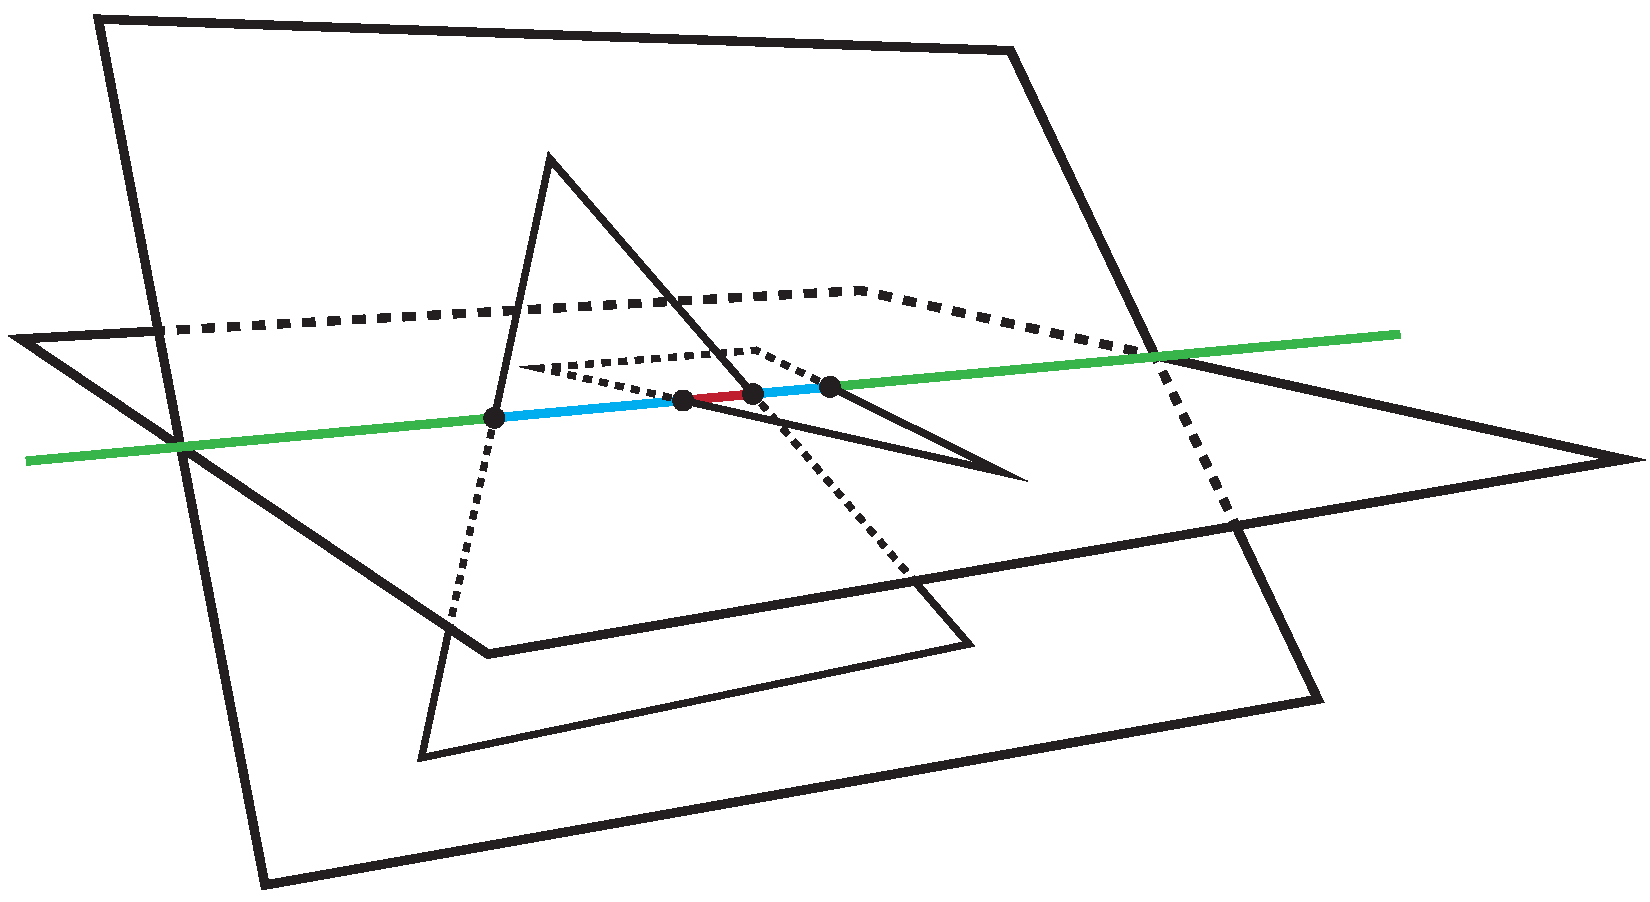
\includegraphics[width=0.8\textwidth]{tri_intersect}
	\caption{
		Intersection line calculation in Möller's triangle intersection test.
		The image shows intervals on the intersection line between two triangle's planes.
		The green line is the intersection line of both planes.
		Blue parts of the intersection line are intervals of one triangle.
		The red part is the overlap of both triangle's line intervals, \ie the triangle's intersection.
		Image modeled after \cite[p757]{tri_tri_intersection_moller_image}.
	}
	\label{fig:tri_intersect}
\end{figure}

Extending beyond this concept, a further optimization is to do not use the planes' intersection line to project the triangle's intervals onto, but to use the coordinate system's axis where the intersection line's direction has the largest magnitude.
This greatly simplifies several calculations except the actual points of the intersection segment.
Furthermore, Möller's code additionally handles the case when both triangles are coplanar, \ie the signed distances of the vertices of one triangle to the other triangle's plane are almost zero.



\subsection{Triangle splitting}
\label{sec:triangle_splitting}

After two structures have been intersected and all intersection lines per triangle have been recorded, the triangles can be split.
The result of splitting a triangle must be a new set of triangles in order to create a new structure from these which can be put into the \textproc{UnionStructure} routine again.
Hence, an algorithm for triangulating a triangle with respect to a set of lines is needed.
In the context of triangulations, this set of lines is usually called constraints or constrained edges and the according algorithm a constrained triangulation (CT).
Initially, a manually written CT was used.
Even though it was capable of triangulating simple cases, it suffered severely from numerical instability and poor output quality.
A stricter triangulation of higher quality is the constrained Delaunay triangulation (CDT), which is also suggested by the paper giving the initial idea to this approach \cite{mesh_intersection}.
However, as CDT algorithms are quite hard to implement regarding speed and robustness, using an established and tested library is highly recommended.
A list of C/C++ libraries offering constrained Delaunay triangulations is given in table \ref{tbl:delaunay_libs}. Several of these libraries have been tested for their suitability to retriangulate a triangle with a set of constraints.
Usually, these triangulation algorithms operate on 2-dimensional point clouds with optional constrained edges between points of this cloud.
As output they generate a Delaunay mesh, with the convex hull of the point cloud as boundary.

\renewcommand{\arraystretch}{1.5} % row spacing
\begin{table}[h]
	\centering
	\begin{tabular}{p{3cm} l l p{2.1cm} p{3.9cm}}
		Library & & Language & License & Notes \\
		\hline
		poly2tri & \cite{poly2tri} & C++ & BSD & Constrains via polylines must not touch each other \\
		Triangle & \cite{triangle_lib} & C & Custom, free for non-commercial use & Difficult interface and memory management \\
		Geometric Tools Engine (GTE) & \cite{gte} & C++ & Boost License & modern C++11, SIMD and GPGPU support, high standard documentation \\
		Computational Geometry Algorithms Library (CGAL) & \cite{cgal_triangulation} & C++ & LGPL, GPL or commercial & Huge functionality, de-facto standard in academics \\
		Fade2D & \cite{fade2d} & C++ & Commercial, free for scientific research & Closed source \\
		Triangulation Template Library (TTL) & \cite{ttl} & C++ & GPL & Supports usage of own data structures via C++ templates \\
		GNU Triangulated Surface Library (GTS) & \cite{gts} & C & LGPL & object-oriented design using GLib\\
		
	\end{tabular}
	\caption{
		Table containing several libraries offering a constrained Delaunay triangulation.
	}
	\label{tbl:delaunay_libs}
\end{table}
\renewcommand{\arraystretch}{1.0}

The poly2tri library requires constraints to be specified as polylines which may not touch each other.
This is a problem as constraints may touch the boundary of the original triangle.
%
The Triangle library has been used for exactly this purpose in another paper \cite{mesh_intersection}.
Nevertheless, it has a very difficult C interface which tries to mimic a command line with text arguments even on API level.
Furthermore, passing in and returning geometric data structures requires extensive care regarding memory management.
The library did work for most of the cases but crashed several times, \eg on every 1000\textsuperscript{th} triangle.  
%
The Geometric Tools Engine (GTE) is a rather modern library with an excellent C++ interface.
The algorithms' precision may be configured via templates.
The library runs outstandingly stable with only a few troubles in cases where the input was numerically problematic, \eg contained points with differences only at the last few digits representable with double precision.
However, these issues can be fixed with appropriate preprocessing of the input, \cf section \ref{sec:numeric_improvements}.
Furthermore, the GTE library is licensed under the Boost License and therefore perfectly usable in commercial products like the VML.
%
The remaining libraries have not been further tested, mainly for the reason that the VML is a commercial product and the use of these libraries would require to drop the code again later.
%
The integration of the GTE's CDT is given in algorithm \ref{alg:triangle_splitting}.

\begin{algorithm}
	\centering
	\begin{algorithmic}[1]
		\Function{SplitTriangle}{$\var{t}, \var{lines}$}
			\State $\var{points} \gets \{\var{t.a}, \var{t.b}, \var{t.c}\}$ \Comment{Order of elements must remain}
			\ForAll{$\var{(p_1, p_2)} \in \var{lines}$}
				\State $\var{points} \gets \var{points} \cup \{\var{p_1}, \var{p_2}\}$
			\EndFor
			\State $\var{cdt} \gets \var{ConstrainedDelaunay2()}$
			\ForAll{$(\var{p_1}, \var{p_2}) \in \var{lines}$}
				\State $\var{cdt.Insert}((\var{points.indexof}(\var{p_1}), \var{points.indexof}(\var{p_2})), \dots)$
			\EndFor
			\State $\var{cdt}(|\var{points}|, \var{points}, \epsilon)$
			
			\State $\var{indices} \gets \var{cdt.GetIndices()}$
			\State $\var{triangles} \gets \varnothing$
			\For{$\var{i} \gets 0,\dots,\frac{|\var{indices}|}{3} - 1$}
				\State $\var{f} \gets \var{triangle()}$
				\For{$\var{j} \gets 0,1,2$}
					\State $\var{index} \gets \var{indices_{i * 3 + j}}$
					\State $\var{f_j} = \var{points_{index}}$
				\EndFor
				%\If{$\var{f.normal} * \var{t.normal} < 0$}
				%	\State $\var{swap}(\var{f.a}, \var{f.b})$ \Comment{Swap two vertices to reverse winding}
				%\EndIf
				\State $\var{triangles} \gets \var{triangles} \cup \{\var{f}\}$
			\EndFor
			\State \Return $\var{triangles}$
		\EndFunction
	\end{algorithmic}
	\caption{
		Adapter to the constrained Delaunay triangulation routine provided by the GTE library.
	}
	\label{alg:triangle_splitting}
\end{algorithm}





\subsection{Triangle inside structure test}
\label{sec:triangle_inside_test}



\subsection{Numeric improvements}
\label{sec:numeric_improvements}

mostly makeRobustChains()


\subsection{Parallelization}
\label{sec:parallelization}


per cell is easy.
at cell level, structure union is a tree-shaped reduction
at union level, triangle-triangle intersections may run fully parallel for each triangle pair, elimination may run fully parallel




\section{Results}
\label{sec:direct_intersection_results}

Why it does not work on larger meshes?
Run time complexity
Numerical robustness

